\documentclass[10pt]{report}
\usepackage{/Users/bradenhoagland/latex/math}


\lhead{Braden Hoagland}
\chead{Differential Geometry}
\rhead{}

\begin{document}
\tableofcontents

%+-------------------+
%| +---------------+ |
%| |    Chapter    | |
%| +---------------+ |
%+-------------------+
% Basics and Tools

\chapter{Basics and Tools}

%%%%%%%%%%%%%%%%%%%%
% Differentiable Functions
%%%%%%%%%%%%%%%%%%%%

\section{Differentiable Functions}

The \textbf{coordinate functions} are maps from $\mathbb{R}^n$ to $\mathbb{R}$, essentially picking out a single coordinate. They are given by
\begin{align*}
	x_i : \mathbb{R}^n &\to \mathbb{R} \\
	\mathbf{p}&\mapsto \mathbf{p}_i.
\end{align*}
If I'm working in $\mathbb{R}^3$, I'll probably use $x,y,$ and $z$ instead of $x_1, x_2,$ and $x_3$.

We say that a function $f:\mathbb{R}^n \to \mathbb{R}$ is \textbf{differentiable} if $f$ can be written as $f(x_1, x_2, \dots, x_n)$ and all partial derivatives of all orders exist and are continuous, i.e. $f$ is $C^{\infty}$. A differentiable function is also called a \textbf{scalar field}.

The set of all differentiable functions/scalar fields forms a ring, so we can perform basic arithmetic with them.

%%%%%%%%%%%%%%%%%%%%
% Surfaces and Manifolds
%%%%%%%%%%%%%%%%%%%%

\section{Surfaces and Manifolds}

{\color{red}Figure out where to put manifolds!!!!}

\begin{defn}[]
A \textbf{manifold} is a set of ``points" $M$ with a collection of ``patches" $\mathcal{P}$. A \textbf{patch} $\mathbf{x} \in \mathcal{P}$ is a one-to-one regular map
\[
\mathbf{x}:\mathcal{D}\to M,
\] where $\mathcal{D}$ is open in $\mathbb{R}^n$. {\color{red}It is \textbf{proper} if $\mathbf{x}^{-1}:\mathbf{x}(\mathcal{D})\to \mathcal{D}$ is continuous.} $M$ and $\mathcal{P}$ satisfy:
\begin{enumerate}
	\item The covering axiom: the images of $\mathcal{P}$ cover $M$.
	\item Smooth overlaps: for all $\mathbf{x},\mathbf{y} \in \mathcal{P}$, the functions $\mathbf{y}^{-1}\mathbf{x}$ and $\mathbf{x}^{-1}\mathbf{y}$ are differentiable in $\mathbb{R}^n$ on their overlap.
	\item $M$ is Hausdorff.
\end{enumerate}
\end{defn}

Because $M$ has a topological restriction, we define the topology on $M$ as the topology generated by the basis
\[
	\mathcal{B} = \left\{ \mathbf{x}(U) \;|\; \mathbf{x} \in \mathcal{P},\; U \text{ open in } \mathcal{D}_{\mathbf{x}} \subset \mathbb{R}^n \right\}.
\] 
A \textbf{surface} is just a 2-dimensional manifold, i.e. it has 2-dimensional patches.

{\color{red}Show that the topology of a surface embedded in $\mathbb{R}^3$ is the subspace topology.}

\begin{ex}[]
The $n$-sphere is a $n$-dimensional manifold.
\end{ex}

\begin{ex}[]
	The tangent bundle $T(M)$ of a surface $M$ is a 4-dimensional manifold. The first two coordinates of its patches represent points on $M$, and the second two represent the coordinates of a point in a particular tangent space of $M$. {\color{red}Does this generalize to $n^2$?}
\end{ex}

%%%%%%%%%%%%%%%%%%%%
% Curves
%%%%%%%%%%%%%%%%%%%%

\section{Curves}

\begin{defn}
A \textbf{curve} in $M$ is a differentiable function $\alpha:I\to M$, where $I$ is an open interval in $\mathbb{R}$.
\end{defn}

Although curves could be defined without the condition that $I$ is open, it makes defining derivatives easier. Without open intervals, we'd have edge cases where some derivatives need to be defined with one-sided limits, and we'd rather just avoid that altogether.
\pagebreak

\begin{ex}
	To draw a helix, we can parameterize a curve $\alpha:\mathbb{R}\to \mathbb{R}^3$ by 
	\[
		\alpha(t)=(a \cos t, a \sin t, bt),
	\] where $a, b\neq 0$.
\end{ex}

\begin{defn}
	Let $\alpha:I\to \mathbb{R}^n$ be a curve. Then for all $t \in I$, the \textbf{velocity} $\alpha'(t)$ is the derivative of $\alpha$ at $t$.
\end{defn}

\begin{figure}[H]
	\centering
	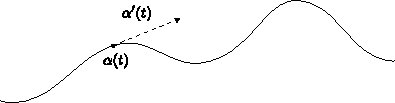
\includegraphics[scale=1]{fig/velocity.pdf}
	\caption{The velocity $\alpha'(t)$ is a vector tangent to $\alpha(t)$.}
\end{figure}

\begin{ex}
Using the parameterization of a helix from the previous example, its velocity vector is
\[
	\alpha'(t) = (-a \sin t, a \cos t, b)_{\alpha(t)}.
\]
\end{ex}

The velocity of a curve isn't determined by the shape of the curve, but rather by how quickly you travel the curve. To illuminate this, we consider reparameterizations of the same curve.

\begin{defn}
	Let $I$ and $J$ be open intervals, let $\alpha:I\to M$ be a curve, and let $h:J\to I$ be differentiable. Then the curve $\beta:J\to M$ given by the composition $\beta = \alpha \circ h$ is called a \textbf{reparameterization} of $\alpha$ by $h$.
\end{defn}

Let $\beta$ be a reparameterization of $\alpha$ by $h$. Then by the chain rule, its velocity vector is
\[
	\beta'(s) = h'(s) \alpha'(h(s)).
\] 
From this we see that unless $h$ has a constant derivative of 1, the velocities of $\alpha$ and $\beta$ will be different at the same point, even though they describe the same curve.

\begin{prop}
Let $\alpha$ be a curve in $\mathbb{R}^n$, and let $f:\mathbb{R}^n\to \mathbb{R}$ be differentiable. Then
\[
	a'(t)[f] = \frac{d (f(\alpha))}{d t} (t).
\] 
\end{prop}
\begin{proof}
	{\color{red}Go over this and fix $\mathbb{R}^n$ to $M$.}
\end{proof}

A curve $\alpha:I\to M$ is \textbf{periodic} if there is some $p>0$ such that $\alpha(t+p) = \alpha(t)$ for all $t$. The smallest such $p$ is then called the \textbf{period} of $\alpha$. A curve whose velocity is nonzero at all points is called \textbf{regular}.

The \textbf{speed} of a curve is
\[
	v(t) = \Vert{\alpha'(t)}\Vert.
\] 

The \textbf{arc length} function (starting from a constant $t=a$) is then defined
\[
	s(t) = \int_{a}^{t} \Vert{\alpha'(\tau)}\Vert\;d\tau.
\] 
From this we have $ds/dt = \Vert{\alpha}\Vert=v$ and $\int_{a}^{b} ds = \int_{a}^{b} \Vert{\alpha'(t)}\Vert\;dt$.

{\color{red}$ds = \Vert{\alpha'(t)}\Vert\;dt$?}

\begin{thrm}[]
We can reparameterize any regular curve $\alpha$ to have unit speed.
\end{thrm}

We say that a unit speed curve has the \textbf{arc length parameterization}.

%+-------------------+
%| +---------------+ |
%| |    Chapter    | |
%| +---------------+ |
%+-------------------+
% Tangent Spaces

\chapter{Tangent Spaces}

%%%%%%%%%%%%%%%%%%%%
% Basics
%%%%%%%%%%%%%%%%%%%%

\section{Basics}

\begin{defn}
	Let $\mathbf{p} \in M$. Then the \textbf{tangent space} $T_\mathbf{p}(M)$ of $M$ at $\mathbf{p}$ is the vector space of all velocities of curves in $M$ originating at $\mathbf{p}$. The \textbf{tangent bundle} $T( M)$ of $M$ is the collection of all tangent spaces of $M$.
\end{defn}

%%%%%%%%%%%%%%%%%%%%
% Vector Fields
%%%%%%%%%%%%%%%%%%%%

\section{Vector Fields}

\begin{defn}
	A \textbf{vector field} $V$ on $M$ is a function
	\[
		V:M \to T_{\mathbf{p}}(M).
	\] 
\end{defn}

Vector fields can be added and scalar multiplied in the usual way for functions. We can also define a notion of vector fields on curves.

\begin{defn}[]
	A \textbf{vector field} on a curve $\alpha:I\to M$ is a function
	\[
		Y: I \to T_{\alpha(t)}(M).
	\]
\end{defn}

A vector field $Y=(y_1, \dots, y_n)$ on a curve $\alpha$ can be decomposed into
\[
	Y = \sum y_i E_i(\alpha).
\] 

We can then define the derivative of a vector field on a curve in a pointwise fashion:
\[
	Y' = \sum y_i' E_i(\alpha).
\] 

A vector field on a curve is \textbf{parallel} if it produces parallel vectors. This means that all of it's $y_i$ are constant.

\begin{prop}
	{\color{red}Move first two statements to curve section? Why are they here?}
	\begin{enumerate}
		\item $\alpha$ is constant $\iff$ $\alpha'=0$.
		\item $\alpha$ is a nonconstant straight line $\iff$ $\alpha''=0$.
		\item $Y$ is parallel $\iff$ $Y'=0$.
	\end{enumerate}
\end{prop}


%%%%%%%%%%%%%%%%%%%%
% 1-Forms
%%%%%%%%%%%%%%%%%%%%

\section{1-Forms}

The derivative $Df_{x}$ of $f$ at $x$ is a linear function that best approximates $f$ at $x$. Note that $Df_{x}$ is a linear function from the tangent space based at $x$ to $\mathbb{R}$ l. 1-forms are a generalization of total derivatives.

\begin{defn}
A \textbf{1-form} on $M$ is a linear function
\[
	\phi:T(M)\to \mathbb{R},
\] such that for all $\mathbf{p}$, we can limit $\phi$ to
\[
	\phi_\mathbf{p}:T_{\mathbf{p}}(M)\to \mathbb{R}.
\] 
\end{defn}

There's an equivalent way of formulating this that uses fancier vocab. If $\mathcal{V}$ is a vector space, then the set of all linear maps from $\mathcal{V}$ to $\mathbb{R}$ is itself a vector space. We call it the \textbf{dual space} of $\mathcal{V}$ and denote it by $\mathcal{V}^*$, and its elements are called \textbf{covectors}.

Thus a 1-form $\phi$ is an element of $T^*(\mathbb{R}^n)$. It can be limited to elements $\phi_\mathbf{p}$ of the \textbf{cotangent space} $T_{\mathbf{p}}^*(\mathbb{R}^n)$, in which case we can also call $\phi_\mathbf{p}$ a \textbf{cotangent vector}.

\begin{note}
Since vector fields produce tangent vectors and 1-forms map tangent vectors to real numbers, we can think of 1-forms as being dual to the notion of vector fields.
\end{note}

Addition of 1-forms is defined pointwise. We can also define a sort of scalar multiplication with scalar fields. If $\phi$ is a 1-form and $f$ is a scalar field, define
\[
	(f\phi)(\mathbf{v}_{\mathbf{p}}) \doteq f(\mathbf{p}) \phi(\mathbf{v}_\mathbf{p})
\] for all $\mathbf{v}_{\mathbf{p}} \in T_\mathbf{p}(\mathbb{R}^n)$.

Given a vector field $V$, we can naturally act on it with a 1-form $\phi$ by
\begin{align*}
	\phi(V):M&\to \mathbb{R} \\
	\mathbf{p}&\mapsto \phi(V(\mathbf{p})).
\end{align*}
Thus we can view 1-forms as operators that convert vector fields into scalar fields. Additionally, it is easy to show that 1-forms act linearly on vector fields.

\begin{defn}
Let $f:M\to \mathbb{R}$ be differentiable. Then the \textbf{differential} $df$ of $f$ is the 1-form such that
\[
	df(\mathbf{v}_{\mathbf{p}}) = \mathbf{v}_{\mathbf{p}}[f]
\] for all tangent vectors $\mathbf{v}_{\mathbf{p}}$ of some point $\mathbf{p} \in M$.
\end{defn}

{\color{red}More on this...}


%%%%%%%%%%%%%%%%%%%%
% Frames
%%%%%%%%%%%%%%%%%%%%

\section{Frames}

\begin{defn}[]
A set of vector fields $\left\{ E_i \right\}_{i=1}^n$ on $M$ if a \textbf{frame} if
\[
\left\langle E_i, E_j \right\rangle = \delta_{ij}.
\] The \textbf{dual frame} is the set of one forms $\left\{ \theta_i \right\}_{i=1}^n$ such that
\[
	\theta_i(E_j) = \delta_{ij}.
\]
\end{defn}

A frame is used to create the ``axes" of each tangent space, and the dual frame is used to project onto each axis. We can explicitly represent the dual frame by
\[
	\theta_i = \left\langle E_i, \;\cdot\; \right\rangle.
\] 

\begin{ex}[]
	If $U_i(\mathbf{p})$ returns a vector with 1 in the $i$-th coordinates and 0 everywhere else, then $\left\{ U_i \right\}_{i=1}^n$ is the \textbf{natural frame field} on $M$. The functions $\left\{ dx_{i} \right\}_{i=1}^n$ are the corresponding dual frame. Thus we can interpret $dx_i$ as simply extracting the $ i$-th component of a tangent vector.
\end{ex}

\begin{prop}
Any 1-form $\phi$ can be written in terms of a frame by
\[
	\phi = \sum \phi(E_i) \theta_i.
\] 
\end{prop}

Here we're saying that $\phi$ is uniquely determined by what it does on the elements of the frame. In the special case that $\phi = df$ for some function $f$ and we're working with the natural frame field, this reduces to
\[
df = \sum \frac{\partial f}{\partial x_i} dx_i.
\] 

\begin{prop}
Any vector field $V$ can be written in terms of a frame by
\[V = \sum \theta_i(V) E_i = \sum \left\langle V,E_i \right\rangle E_i.\]
\end{prop}

Then the inner product of two vector fields $V,W$ is
\[
	\left\langle V,W \right\rangle = \sum \theta_i(V) \theta_i(W) = \sum \left\langle E_i, V \right\rangle \left\langle E_i, W \right\rangle.
\] 


%%%%%%%%%%%%%%%%%%%%
% Directional Derivatives
%%%%%%%%%%%%%%%%%%%%

\section{Directional Derivatives}

{\color{red}Generalize and move to `Basics' section.}

\begin{defn}
	Let $f:\mathbb{R}^n \to \mathbb{R}$ be a scalar field, and let $\mathbf{v}_{\mathbf{p}} \in T_p(\mathbb{R}^n)$. Then
	\[
		\mathbf{v}_{\mathbf{p}}[f] \doteq \frac{d }{d t} f(\mathbf{p}+t\mathbf{v}) \Big|_{t=0}
\] is the \textbf{directional derivative} of $f$ at $\mathbf{p}$ in the direction of $\mathbf{v}$. Note that it is a real number.
\end{defn}

\begin{prop}
	\label{prop:dir-der}
	Let $\mathbf{v}_\mathbf{p} \in T_\mathbf{p}(\mathbb{R}^n)$, then
	\[
		\mathbf{v}_{\mathbf{p}}[f] = \sum_i v_i \frac{\partial f}{\partial x_i} (\mathbf{p}).
	\] 
\end{prop}
\begin{proof}
	Since $\frac{d }{d t} (p_i + tv_i) = v_i$, we can use the chain rule to get
	\begin{align*}
		\frac{d }{d t} f(\mathbf{p}+t\mathbf{v}) \Big|_{t=0} &= \sum_{i} v_i \frac{\partial f}{\partial x_i} (\mathbf{p}+t\mathbf{v}) \Big|_{t=0} \\
						   &= \sum_i v_i \frac{\partial f}{\partial x_i} (\mathbf{p}).
	\end{align*}
\end{proof}

\begin{thrm}
	\label{thrm:props-of-dir-der}
	Let $f,g:\mathbb{R}^n \to \mathbb{R}$ be scalar functions, let $\mathbf{v},\mathbf{w} \in T_\mathbf{p}(\mathbb{R}^n)$, and let $\lambda,\eta\in\mathbb{R}$, then
	\begin{enumerate}
		\item $(\lambda \mathbf{v} + \eta \mathbf{w})[f] = \lambda \mathbf{v}[f] + \eta \mathbf{w}[f]$,
		\item $\mathbf{v}[\lambda f + \eta g] = \lambda \mathbf{v}[f] + \eta \mathbf{v}[g]$, and
		\item $\mathbf{v}[fg] = \mathbf{v}[f] g(\mathbf{p}) + f(\mathbf{p}) \mathbf{v}[g]$.
	\end{enumerate}
\end{thrm}
\begin{proof}
	It's straightforward to prove these by using Proposition \ref{prop:dir-der}.
\end{proof}

Parts (1) and (2) of this theorem say that $\mathbf{v}[f]$ is linear in both $\mathbf{v}$ and $f$. Part (3) is just the Leibniz rule.

It's easy to extend this idea to use a vector field instead of a fixed tangent vector. We simply use the vector field to map to a tangent vector, then use that to construct a directional derivative.

\begin{note}
In this sense, vector fields map scalar fields to other scalar fields.
\end{note}

\begin{defn}
	The \textbf{operator} of a vector field $V$ on a scalar field $f$ is itself a scalar field
	\begin{align*}
		V[f]: \mathbb{R}^n &\to \mathbb{R} \\
		\mathbf{p} &\mapsto V(\mathbf{p})[f].
	\end{align*}
\end{defn}

\begin{ex}
If $\left\{ U_i \right\}_{i=1}^n$ is the natural frame field on $V$, then $U_i[f] = \frac{\partial f}{\partial x_i} .$
\end{ex}

\begin{cor}
	Let $V,W$ be vector fields on $\mathbb{R}^n$, let $f,g,h:\mathbb{R}^n \to \mathbb{R}$ be scalar fields, and let $\lambda,\eta \in \mathbb{R}$, then
	\begin{enumerate}
		\item $(fV+gW)[h] = fV[h] + gW[h]$,
		\item $V[\lambda f+\eta g] = \lambda V[f] + \eta V[g]$, and
		\item $V[fg] = V[f] g + f V[g]$.
	\end{enumerate}
\end{cor}
\begin{proof}
	It's straightforward to prove these by using the corresponding part of Theorem \ref{thrm:props-of-dir-der}.
\end{proof}

Note that a ``scalar" in part (1) of this corollary can be a function, but the scalars must be actual numbers in part (2). That's because in part (1), the functions $f$ and $g$ get evaluated at some point $\mathbf{p}$, which yields a real number. In part (2), the only thing that gets evaluated at $\mathbf{p}$ is $V$, not anything in brackets.


%%%%%%%%%%%%%%%%%%%%
% The Covariant Derivative
%%%%%%%%%%%%%%%%%%%%

\section{The Covariant Derivative}

The covariant derivative is how we measure the rate of change of a vector field in a particular direction. {\color{red}Comparison to $Y'$ from vector field on curve?}

{\color{red}Compare this definition to that in the book...}

\begin{defn}[]
	Let $\mathbf{v} \in T_{\mathbf{p}}$, then the \textbf{covariant derivative} of a vector field $W$ with respect to $\mathbf{v}$ is
	\[
		\nabla_{\mathbf{v}}W = \frac{d }{d t} W(\mathbf{p}+t\mathbf{v})\Big|_{t=0}.
	\] 
\end{defn}

If $W = \sum w_i U_i$, then this can be written
\begin{align*}
	\nabla_{\mathbf{v}}W &= \sum \left( \nabla_{\mathbf{v}}W \cdot U_i(\mathbf{p}) \right) U_i(\mathbf{p}) \\
			     &= \sum \mathbf{v}[w_i]U_i(\mathbf{p}).
\end{align*}

{\color{red}Linearity and all that.}

We can easily extend this to being based on another vector field instead of a single tangent vector. If $V$ and $W$ are vector fields, then
\[
	\nabla_{V}W(\mathbf{p}) = \nabla_{V(\mathbf{p})}W.
\] If $W = \sum w_i U_i$, then $\nabla_{V}W = \sum V[w_i] U_i$.

Since $\nabla_{V}W$ maps from $\mathbb{R}^n$ to $T_{\mathbf{p}}(\mathbb{R}^n)$, it is itself a vector field.

{\color{red}Linearity and all that stuff.}


%%%%%%%%%%%%%%%%%%%%
% Differential Forms
%%%%%%%%%%%%%%%%%%%%

\section{Differential Forms}

1-forms are part of a larger family of differential forms. 0-forms are just scalar fields, 1-forms are of the form $\sum f_i \;dx_i$, and we can get all other $n$-forms through multiplication of other forms.

Define the wedge product ... {\color{red}(do this.)} The only unusual rule that the wedge product must follow is anti-commutativity:
\[
\phi \wedge \psi = - \psi \wedge \phi.
\] 

\begin{ex}
A direct consequence of anti-commutativity is that two 1-forms wedged together is the zero map:
\[
\phi\wedge\phi = 0.
\] 
\end{ex}

\begin{note}
I might write $dx_i \wedge dx_j$ as $dx_i\;dx_j$ for simplicity.
\end{note}

{\color{red}explicit form for evaluating a 2-form (pg 160)... also just more on this in general...}

We can generalize the differential to apply to more than just scalar fields (0-forms). Given any form
\[
\varphi = \sum_{I} f_I \;dx_I,
\] we define $d\varphi$ by
\[
	d\varphi \doteq \sum_{I} d(f_I)\wedge \;dx_I.
\] 
Thus we can view the $d$ operator as converting an $n$-form to an $(n+1)$-form, and we call it the \textbf{exterior derivative}. If we denote the space of $n$-forms on $M$ by $\Omega_n(M)$, this gives us the following cochain complex.
\begin{figure}[H]
	\centering
\begin{tikzcd}
0 \arrow[r, "d"] & \Omega_1(M) \arrow[r, "d"] & \Omega_2(M) \arrow[r, "d"] & \Omega_3(M) \arrow[r, "d"] & \cdots
\end{tikzcd}
\end{figure}
A form $\phi$ is \textbf{closed} if $d\phi=0$, and it is \textbf{exact} if $\phi = d\varphi$ for some form $\varphi$.

%+-------------------+
%| +---------------+ |
%| |    Chapter    | |
%| +---------------+ |
%+-------------------+
% Euclidean Geometry

\chapter{Euclidean Geometry}

%%%%%%%%%%%%%%%%%%%%
% The Cross Product
%%%%%%%%%%%%%%%%%%%%

\section{The Cross Product}

For $\mathbf{v}, \mathbf{w} \in T_{\mathbf{p}}(\mathbb{R}^3)$, we define the cross product as
\[
\mathbf{v} \times \mathbf{w} = \left| 
\begin{matrix}
	U_1(\mathbf{p}) & U_2(\mathbf{p}) & U_3(\mathbf{p}) \\
	v_1 & v_2 & v_3 \\
	w_1 & w_2 & w_3
\end{matrix}\right|.
\] 

{\color{red}Interpretation as signed area?}

The cross product is linear in $\mathbf{v}$ and $\mathbf{w}$, and it satisfies the alternation rule
\[
\mathbf{v} \times \mathbf{w} = -\mathbf{w}\times \mathbf{v},
\] so any vector crossed with itself is $\mathbf{0}$.

The cross product produces a vector that is orthogonal to $\mathbf{v}$ and $\mathbf{w}$, so
\[
	\mathbf{v} \cdot (\mathbf{v}\times \mathbf{w}) = \mathbf{w}\cdot (\mathbf{v}\times \mathbf{w}) = 0.
\] 

{\color{red}$\varepsilon$ stuff and experssion in terms of $\sin$.}

%%%%%%%%%%%%%%%%%%%%
% The Frenet Formulas
%%%%%%%%%%%%%%%%%%%%

\section{The Frenet Formulas}

We start out by describing a particular frame on a curve that ends up being very helpful. The core idea behind this is that we can take derivatives to find tangent and normal components of the frame, then take their cross product to get a third orthogonal component. This constitutes a frame that changes based on the curve's geometry at each point.

Suppose $\beta$ is a unit speed curve in $\mathbb{R}^3$. Then $T\doteq\beta'$ is the \textbf{unit tangent vector field}. Since $\beta$ is unit speed, $\Vert{T}\Vert=1$ everywhere, so it needs no further modifications to be a part of our frame.

Since $\Vert{T}\Vert^2 = T\cdot T=1$, we differentiate to get $2(T'\cdot T)=0$, so its derivative is orthogonal to it. The normalized version of this field will be the next component of our frame. Define the \textbf{curvature} of $\beta$ by $\kappa(s) = \Vert{T'(s)}\Vert\geq 0$, then when $\kappa > 0$, define $N = T' / \kappa$ to be the \textbf{principal normal vector field}.

Finally, define $\beta = T \times N$ to be the \textbf{binormal vector field}. {\color{red}Cross two units = unit.} In summary, the \textbf{Frenet apparatus} is
\begin{itemize}
	\item $T=\alpha'$,
	\item $\kappa = \Vert{\alpha'}\Vert$,
	\item $N = T' / \kappa$, and
	\item $B = T \times N$.
\end{itemize}
\begin{defn}[]
	For a unit speed curve $\beta$ with $\kappa>0$ everywhere, $B$, $N$, and $T$ form the \textbf{Frenet frame field} on $\beta$. They constitute a frame at each point on $\beta$.
\end{defn}

\begin{figure}[H]
	\centering
	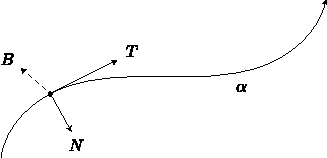
\includegraphics[scale=1.5]{fig/frenet.pdf}
	\caption{The Frenet frame at a particular point on $\alpha$. It's hard to see in 2D, but the $B$ vector is supposed to be coming out of the page.}
\end{figure}

Since $B \cdot B=1$, $B' \cdot B = 0$. Also, $B \cdot T = 0$, so
	\[
	B' \cdot T = -B \cdot T' = -\kappa B \cdot N = 0.
	\]
	Thus $B'$ is orthogonal $T$ and $B$, so it must be parallel to $N$, meaning $B' = -\tau N$ for some $\tau$ (the negative sign is convention). This $\tau$ is called the \textbf{torsion}.

\begin{thrm}[The Frenet Formulas]
Let $\beta:I \to \mathbb{R}^3$ be a unit speed curve with nonzero $\kappa$ everywhere and torsion $\tau$, then
\begin{align*}
	T' &= \kappa N, \\
	N' &= -\kappa T + \tau B, \\
	B' &= -\tau N.
\end{align*}
\end{thrm}
\begin{proof}
	{\color{red}Do expansion of $N'$.}
\end{proof}

From this we see that the geometry of a curve is encoded in its curvature and torsion.

{\color{red}Examples...}

\begin{prop}
A curve is a straight line if and only if $\kappa=0$.
\end{prop}
{\color{red}Proof?}

\begin{prop}
 	A unit speed curve with $\kappa>0$ is planar if and only if $\tau = 0$.
\end{prop}
\begin{proof}
	{\color{red}Do this.}
\end{proof}

\begin{lem}
	If $\kappa>0$ and $\kappa'=\tau=0$, then $\beta$ is (part of) a circle of radius $1/\kappa$.
\end{lem}
\begin{proof}
	{\color{red}Do this.}
\end{proof}

%%%%%%%%%%%%%%%%%%%%
% Arbitrary Speed Curves
%%%%%%%%%%%%%%%%%%%%

\section{Arbitrary Speed Curves}

Let $\overline{\alpha} :I\to \mathbb{R}^3$ be a unit speed curve, and let $\alpha=\overline{\alpha}(s)$ be an arbitrary reparameterization. 

We can ``correct" the old Frenet formulas to give formulas that work for our arbitrary curve by simplying multiplying by the speed function $v$. To see this, note that for our new curve $\alpha$,
\[
T' = \frac{d T}{d t} = \frac{d T}{d s} \frac{d s}{d t} = \overline{T}'v.
\] 
The cases for $B'$ and $N'$ are similar.

\begin{thrm}[]
	Let $\alpha$ be an arbitrary regular ($\kappa>0)$) curve, then
\begin{align*}
	T' &= \kappa v N, \\
	N' &= -\kappa v T + \tau v B, \\
	B' &= -\tau v N.
\end{align*}
\end{thrm}

If $\beta$ has constant speed $\Vert{\beta'}\Vert$, then differentiating gives $2(\beta''\cdot \beta') = 0$, so $T$ and $N$ are orthogonal. This might not be the case if the speed of $\beta$ isn't constant, though. {\color{red}Does this mean the Frenet ``frame" isn't a frame when $\alpha$ isn't constant speed?} {\color{red}Are $\beta' and \beta''$ always in correspondence with $T$ and $N$? I assumed so above.}

\begin{lem}
	Let $\alpha$ be a regular curve with speed function $v$, then it's velocity and acceleration are given by
	\begin{align*}
		\alpha' &= vT, \\
		\alpha'' &= v'T + \kappa v^2 N.
	\end{align*}
\end{lem}
\begin{proof}
	The velocity is $\alpha' =\overline{\alpha}'(s)v = \overline{T}(s)v = Tv$. Differentiating gives $\alpha''=v'T + vT'$, which is equal to $v'T + \kappa v^2 N$ by the updated Frenet formulas.
\end{proof}

\begin{figure}[H]
	\centering
	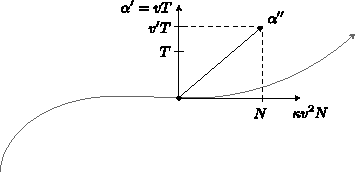
\includegraphics[scale=1.5]{fig/frenet2.pdf}
	\caption{The above lemma is just saying that acceleration along a curve can be decomposed into tangential and centripetal components.}
\end{figure}


\begin{thrm}[]
We can express the Frenet apparatus as
\begin{gather*}
	T = \frac{\alpha'}{\Vert{\alpha'}\Vert} ,\quad\quad N = B \times T,\quad\quad B = \frac{\alpha' \times \alpha''}{\Vert{\alpha' \times \alpha''}\Vert} ,\\
	\kappa = \frac{\Vert{\alpha' \times \alpha''}\Vert}{\Vert{\alpha'}\Vert^3} ,\quad\quad \tau = \frac{(\alpha' \times \alpha'')\cdot \alpha'''}{\Vert{\alpha'\times \alpha''}\Vert^2} .
\end{gather*}
\end{thrm}
\begin{proof}
	{\color{red}Do this.}
\end{proof}

%%%%%%%%%%%%%%%%%%%%
% Connection Forms
%%%%%%%%%%%%%%%%%%%%

\section{Connection Forms}

The Frenet formulas were powerful because they expressed the derivatives of the Frenet frame field in terms of itself. We now generalize this by expressing the covariant derivative of any frame field in terms of the frame field itself.

We showed earlier that we can decompose the covariant derivative based on the natural frame field. It's easy to extend this to work with any frame field instead. For any $\mathbf{v} \in T_{\mathbf{p}}$,
\[
	\nabla_{\mathbf{v}}E_i = \sum_j \omega_{ij}(\mathbf{v}) E_j(\mathbf{p}),
\] where $\omega_{ij}(\mathbf{v}) = \nabla_{\mathbf{v}}E_i \cdot E_{j}(\mathbf{p})$ is a scalar. It's easy to extend this to work with entire vector fields $V$ instead of particular vectors $\mathbf{v}$:
\[
	\nabla_{V}E_i = \sum_j \omega_{ij}(V) E_j,
\] where $\omega_{ij}$ is composed with $V$ in the usual way for functions.

{\color{red}\[
		\omega_{ij}(V) = \left\langle \nabla_{V}E_i, E_j \right\rangle.
\] }

\begin{defn}[]
We call the $\omega_{ij}$ the \textbf{connection forms} of $\left\{ E_1, \dots, E_n \right\}$.
\end{defn}

\begin{lem}
	Each $\omega_{ij}$ is a 1-form. Also, $\omega_{ij}=-\omega_{ji}$.
\end{lem}
\begin{proof}
	$\omega_{ij}$ is a function from $T_{\mathbf{p}}(\mathbb{R}^n)$ to $\mathbb{R}$, and its linearity follows from that of the covariant derivative:
	\begin{align*}
		\omega_{ij}(a\mathbf{v} + b\mathbf{w}) &= (\nabla_{a\mathbf{v} + b\mathbf{w}}E_i) \cdot E_j \\
						       &= (a \nabla_{\mathbf{v}}E_i\cdot + b\nabla_{\mathbf{w}}E_i)\cdot E_j \\
						       &= a\omega_{ij}(\mathbf{v})+b\omega_{ij}(\mathbf{w}).
	\end{align*}
	Since $E_i \cdot E_j = \delta_{ij}$ is a constant, its derivative in any direction is 0. Then
	\[
		0 = \mathbf{v}[E_i \cdot E_j] = \nabla_{\mathbf{v}}E_i(\mathbf{p})\cdot E_j + E_i \cdot \nabla_{\mathbf{v}}E_j(\mathbf{p}) = \omega_{ij}(\mathbf{v}) + \omega_{ji}(\mathbf{v}),
	\]
	so $\omega_{ij}=-\omega_{ji}$.
\end{proof}

This antisymmetry means that we can gather all the $w_{ij}$ into an antisymmetric matrix. In 3 dimensions, we can express the covariant derivatives of $E_1,E_2,E_3$ by the system
\[
	\nabla_{V}
	\begin{pmatrix}
		E_1\\E_2\\E_3
	\end{pmatrix}=
\begin{pmatrix}
	0 & \omega_{12}& \omega_{13} \\
	-\omega_{12}&0&\omega_{23}\\
	-\omega_{13}&-\omega_{23}&0
\end{pmatrix}
\begin{pmatrix}
	E_1\\E_2\\E_3
\end{pmatrix}.
\] 
So in 3 dimensions, there are only three 1-forms of interest when describing the covariant derivative of a frame field.

We can now express the covariant derivatives of the element of a frame field in terms of matrix multiplication. For example, the Frenet formulas can be written
\[
\frac{d }{d s} 
\begin{pmatrix}
	T \\ N \\ B
\end{pmatrix} = 
\begin{pmatrix}
	0 & \kappa & 0 \\
	-\kappa &0&\tau \\
	0&-\tau&0
\end{pmatrix}
\begin{pmatrix}
	T \\ N \\ B
\end{pmatrix}.
\] 
There are differences, of course, between the Frenet formulas and general connection forms. That biggest is probably that the Frenet formulas allow for $\kappa$ and $\tau$ to be any functions, not just 1-forms. This is because the Frenet formulas need only describe what's going on along a 1-dimensional curve, not an arbitrary vector field.

We can calculate the connection forms of a frame field relatively easily using the attitude matrix from way back when. We originally defined the attitude matrix in terms of just frames, but it's super easy to extend it to work with frame fields instead:
\[
E_i = \sum_j a_{ij}U_j,
\] where $A = [a_{ij}]$ is a matrix of scalar fields. Note that if we plug in a point $\mathbf{p}$, then we recover the same attitude matrix from the original definition.

\begin{thrm}[]
	If $A=[a_{ij}]$ is the attitude matrix and $\omega=[\omega_{ij}]$ is the matrix of connection forms of the frame field $\left\{ E_1,E_2,E_3 \right\}$, then
	\[
	\omega = dA \; A^T.
	\] 
	Equivalently,
	\[
	\omega_{ij} = \sum_k da_{ik}\;a_{jk}.
	\] 
\end{thrm}
\begin{proof}
	{\color{red}Do this.}
\end{proof}

\begin{note}[]
Prof likes to use Einstein summation convention, so that'll probably start popping up every now and then.
\end{note}

{\color{red}Examples...}

%%%%%%%%%%%%%%%%%%%%
% The Cartan Structure Equations
%%%%%%%%%%%%%%%%%%%%

\section{The Cartan Structure Equations}

\begin{ex}[]
	$\theta_i(U_j) = E_i \cdot U_j=a_{ij}$, where $a_{ij}$ is an element of the attitude matrix. Thus if
	\[
	E_i = \sum a_{ij}U_j,
	\] then the dual is
	\[
		\theta_i = \theta_i(U_j) \;dx_j=\sum a_{ij}\;dx_j.
	\] Thus we can use the same attitude matrix to translate from standard to arbitrary bases for both vector fields and 1-forms.
\end{ex}

\begin{thrm}[The Cartan Structure Equations]
	Let $\left\{ E_i \right\}$ be a frame field on $\mathbb{R}^n$. Then the exterior derivatives of the dual forms and connection forms satisfy
\begin{enumerate}
	\item $d\theta_i = \sum_j \omega_{ij}\wedge \theta_j$, or as matrices, $d\theta=\omega\wedge\theta$;
	\item $d\omega_{ij}=\sum_k \omega_{ik}\wedge\omega_{kj}$, or as matrices, $d\omega=\omega\wedge\omega$.
\end{enumerate}
\end{thrm}
\begin{proof}
	{\color{red}Go over this b/c matrices suck.}

	{\color{red}$\theta$ is a column matrix. $\omega$ is a square matrix.}

	{\color{red}Note that $\omega\wedge\omega$ isn't 0 because this is actually noting that we're multiplying two matrices but using the wedge instead of usual multiplication.}
\end{proof}

{\color{red}End of pg 95-pg 98}

%+-------------------+
%| +---------------+ |
%| |    Chapter    | |
%| +---------------+ |
%+-------------------+
% Replace this chapter

\chapter{Replace this chapter}

%%%%%%%%%%%%%%%%%%%%
% Orientation
%%%%%%%%%%%%%%%%%%%%

\section{Orientation}

\begin{defn}[]
	If $f$ is any scalar field on $\mathcal{D}$, then a \textbf{Monge patch} is a function $\mathbf{x}:\mathcal{D}\to \mathbb{R}^3$ of the form $\mathbf{x}(u,v)=(u,v,f(u,v))$.

	A \textbf{simple surface} is a surface that can be covered by a single patch.
\end{defn}

To check that all Monge patches are in fact regular and one-to-one, we compute its Jacobian
\[
\begin{pmatrix}
	1 & 0 & \partial_{u}{f} \\
	0 & 1 & \partial_{v}{f} 
\end{pmatrix}.
\] Since this is full rank, we're all good. {\color{red}one-to-one with matrix?}

\begin{thrm}[]
	Let $g$ be a scalar field on $\mathbb{R}^3$. The subset \[M_c \doteq \left\{ \mathbf{p} \;|\; g(\mathbf{p})=c \right\}\] is a surface if $dg$ is nonzero at any point of $M_c$. {\color{red}Does this mean all or any?}

	{\color{red}Could be empty?}
\end{thrm}
\begin{proof}
	{\color{red}Do this.}
\end{proof}

If $\mathbf{x}:\mathcal{D}\to \mathbb{R}^3$ is a patch, then for fixed $v_0$, the curve
\[u\mapsto \mathbf{x}(u,v_0)\] is a \textbf{$u$-parameter curve} in $M$. The definition of \textbf{$v$-parameter curves} is similar.

\begin{defn}[]
	The \textbf{partial velocities} $\mathbf{x}_{u}$ and $\mathbf{x}_{v}$ of $\mathbf{x}$ at $(u_0,v_0)$ are the velocities along the $u$ and $v$ curves, respectively.
\end{defn}

\begin{defn}[]
	A regular mapping $\mathbf{x}:\mathcal{D}\to \mathbb{R}^3$ whose image lies in $M$ is a \textbf{parameterization} of $\mathbf{x}(\mathcal{D})$.
\end{defn}

Note that a parameterization need not be one-to-one or proper.

%+-------------------+
%| +---------------+ |
%| |    Chapter    | |
%| +---------------+ |
%+-------------------+
% Surfaces in R^3

\chapter{Surfaces in \texorpdfstring{$\mathbb{R}^3$}{R3}}

\begin{note}[]
For the remainder of this chapter, we'll be working with surfaces embedded in $\mathbb{R}^3$.
\end{note}

{\color{red}Make note in curvature section about connectedness assumption...}

%%%%%%%%%%%%%%%%%%%%
% Maps of Surfaces
%%%%%%%%%%%%%%%%%%%%

\section{Maps of Surfaces}

\begin{defn}
The \textbf{tangent map} $F_*$ of a map $F:M\to N$ is a map
\[
	F_* : T(M) \to T(N)
\] between the tangent bundles of $M$ and $N$. In particular, at any point $\mathbf{p}$, the tangent map can be limited to the function
\[
	F_{*\mathbf{p}}:T_{\mathbf{p}}(M)\to T_{F(\mathbf{p})}(N)
\]
given by mapping the initial velocity of a curve $\alpha$ in $M$ to the initial velocity of the curve $F(\alpha)$ in $N$.
\end{defn}

\begin{figure}[H]
	\centering
	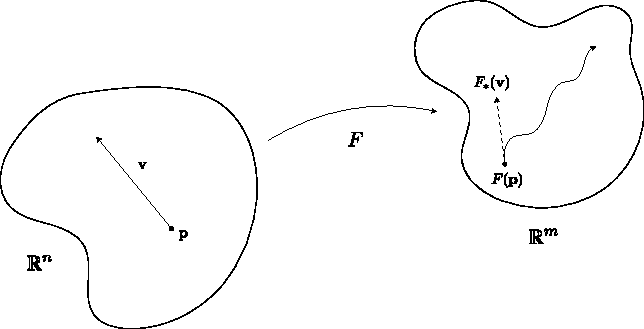
\includegraphics[scale=1]{fig/tan-map.pdf}
	\caption{The tangent map $F_*$ maps tangent spaces to tangent spaces by using the velocity of a curve. {\color{red}Generalize image.}}
\end{figure}

This shows $F_*$ is linear, but it's more than just a linear map between tangent spaces. It's very deeply connected to the {\color{red}more subtle than this, I think...}Jacobian... in the sense that it actually is the Jacobian. The corollary below might look complicated, but all it's saying is that $F_*$ is the linear map given by the matrix $[\frac{\partial f_i}{\partial f_j} ]_{ij}.$

{\color{red}Actually calculate $F_{*\mathbf{p}}(\mathbf{v}_{\mathbf{p}})$. Does it involve multiplying a tangent vector by the Jacobian maybe?}

{\color{red}1-1 iff onto when linear transformation is between two vec spaces of same dim. Useful for showing when $F_{*\mathbf{p}}$ is an isomorphism.}

\begin{note}
We can interpret $F_*$ at $\mathbf{p}$ as the best linear approximation to $F$ at $\mathbf{p}$.
\end{note}

\begin{defn}[]
A mapping $F$ is \textbf{regular} if $F_*$ is one-to-one at all $\mathbf{p}$.
\end{defn}

This isn't the only way to characterize a regular mapping. Since $F_*$ is linear, the following are equivalent:
\begin{enumerate}
	\item $F_*$ is everywhere one-to-one.
	\item $F_*(\mathbf{v}) = 0$ implies $\mathbf{v}=0.$ 
	\item The Jacobian of $F$ is full rank.
\end{enumerate}

\begin{defn}[]
	A \textbf{diffeomorphism} is a mapping that has a differentiable inverse.
\end{defn}

\begin{thrm}[Inverse Function Theorem]
Let $F:\mathbb{R}^n\to \mathbb{R}^n$ be a mapping between Euclidean spaces of the same dimension. If $F_*$ is one-to-one at $\mathbf{p}\in \mathbb{R}^n$, then there is an open neighborhood $U$ of $\mathbf{p}$ such that $F$ restricted to $U$ is a diffeomorphism onto some open set $V$.
\end{thrm}

This is saying that if we have a mapping from $\mathbb{R}^n$ to $\mathbb{R}^n$ that is one-to-one at a given point, then that mapping is locally invertible at that point.


%%%%%%%%%%%%%%%%%%%%
% Pullbacks and Pushforwards
%%%%%%%%%%%%%%%%%%%%

\section{Pullbacks and Pushforwards}

%%%%%%%%%%%%%%%%%%%%
% Integration on Surfaces
%%%%%%%%%%%%%%%%%%%%

\section{Integration on Surfaces}


%%%%%%%%%%%%%%%%%%%%
% Topological Properties
%%%%%%%%%%%%%%%%%%%%

\section{Topological Properties}

%%%%%%%%%%%%%%%%%%%%
% Homotopies
%%%%%%%%%%%%%%%%%%%%

\section{Homotopies}


%%%%%%%%%%%%%%%%%%%%
% Curvature
%%%%%%%%%%%%%%%%%%%%

\section{Curvature}

\begin{defn}[]
The \textbf{shape operator} $S_p$ of a surface $M$ at $\mathbf{p}$ is the linear map
\begin{align*}
	S_p: T_{\mathbf{p}}(M)&\to T_{\mathbf{p}}(M)\\
	\mathbf{v} &\mapsto  -\nabla_{\mathbf{v}}U,
\end{align*}
where $\mathbf{v}$ is tangent to $M$ at $\mathbf{p}$ and $U$ is a unit normal vector field on a neighborhood of $\mathbf{p}$ in $M$.
\end{defn}

There is some ambiguity here, since if $U$ is a unit normal vector field, then so is $-U$. The shape operator is based on $U$, so $-S_{\mathbf{p}}$ is based on $-U$.

The shape operator is symmetric: $S(\mathbf{v}) \cdot \mathbf{w} = S(\mathbf{w})\cdot \mathbf{v}$ for all pairs of tangent vectors of $\mathbf{p}$.

\begin{prop}
If $\alpha$ is a curve in $M \subset \mathbb{R}^3$, then
\[
	\alpha'' \cdot U = S(\alpha') \cdot \alpha'.
\] 
\end{prop}

This motivates the definition of normal curvature, which is a measure of how $M$ is bent in the direction of a unit tangent vector.
\begin{defn}[]
If $\mathbf{u}$ is a unit tangent vector to $M \subset \mathbb{R}^3$ at $\mathbf{p}$, then the \textbf{normal curvature} of $M$ in the $\mathbf{u}$ direction is
\[
	k(\mathbf{u}) = S(\mathbf{u}) \cdot \mathbf{u}.
\] 
\end{defn}

Note that $k(\mathbf{u}) = k(-\mathbf{u})$.

{\color{red}other normal curvature stuff.}

Since $S$ is symmetric, we can diagonalize it. The (unit) eigenvectors $\mathbf{e}_1, \mathbf{e}_2$ of this new matrix are the \textbf{principal directions}, and their respective eigenvalues $k_1,k_2$ are the \textbf{principal curvatures}.

\begin{prop}
	$k_1$ and $k_2$ are the minimum and maximum {\color{red}(respectively?)} normal curvatures.
\end{prop}
\begin{proof}
	{\color{red}Think about this...}
\end{proof}

We say that $\mathbf{p}$ is \textbf{umbilic} if $S_{\mathbf{p}}$ if just multiplies by a scalar, i.e. $k_1=k_2$. This means the normal curvature is constant in all directions at $\mathbf{p}$, so every direction is principal.

If $\mathbf{p}$ is nonumbilic, then the principal diretions are unambiguous. In fact, they are orthongonal {\color{red}(why?)}.

\begin{defn}[]
The \textbf{Gaussian curvature} of $M \subset \mathbb{R}^3$ at $\mathbf{p}$ is
\[
K \doteq \det S_{\mathbf{p}} = k_1 k_2.
\] The \textbf{mean curvature} is
\[
	H \doteq \text{tr}\, S_{\mathbf{p}} = (k_1+k_2)/2.
\] 
\end{defn}

Note that if we use $-U$ instead of $U$, the mean curvature is negated while the Gaussian curvature is left unchanged.

\begin{prop}
	If $\mathbf{v},\mathbf{w} \in T_{\mathbf{p}}(M)$ are linearly independent, then
	\begin{align*}
		S(\mathbf{v}) \times S(\mathbf{w}) &= K(\mathbf{p}) \mathbf{v} \times \mathbf{w}, \\
		S(\mathbf{v}) \times \mathbf{w} + \mathbf{v} \times S(\mathbf{w}) &= 2H(\mathbf{p}) \mathbf{v} \times \mathbf{w}.
	\end{align*}
\end{prop}

{\color{red}Euler formula for normal curvature... (pg 214)}

\end{document}
